\documentclass[12pt, letterpaper]{report}
\usepackage{enumitem}
\usepackage[a4paper, margin=0.7in, top=20mm, bottom=20mm]{geometry}
\usepackage{mathspec}
\usepackage[UTF8]{ctex}
\usepackage[colorlinks=true, linkcolor=black, urlcolor=blue]{hyperref}
\usepackage{listings}
\usepackage{xcolor}
\usepackage{graphicx}
\usepackage{xparse}
\usepackage{tcolorbox}
\usepackage{mdframed}

\graphicspath{ {./pics/} }

% ---- Code Section Style ----
\colorlet{mygray}{black!30}
\colorlet{mygreen}{green!60!blue}
\colorlet{mymauve}{red!60!blue}

\tcbuselibrary{breakable}
\NewDocumentCommand{\exercise}{ m +m }{
    {
        \edef\originalParIndent{\the\parindent}
        \begin{tcolorbox}[breakable,arc=0mm,boxrule=0.8pt]
            \setlength{\parindent}{\originalParIndent}
            \noindent
            \textbf{\large Exercise #1}
            \indent
            #2
        \end{tcolorbox}
    }
}

\tcbuselibrary{breakable}
\NewDocumentCommand{\question}{ m +m }{
    {
        \edef\originalParIndent{\the\parindent}
        \begin{tcolorbox}[breakable,arc=0mm,boxrule=0.8pt]
            \setlength{\parindent}{\originalParIndent}
            \noindent
            \textbf{\large Question}
            \indent
            #2
        \end{tcolorbox}
    }
}

\tcbuselibrary{breakable}
\NewDocumentCommand{\challenge}{ m +m }{
    {
        \edef\originalParIndent{\the\parindent}
        \begin{tcolorbox}[breakable,arc=0mm,boxrule=0.8pt]
            \setlength{\parindent}{\originalParIndent}
            \noindent
            \textbf{\large Challenge!}
            \indent
            #2
        \end{tcolorbox}
    }
}

\lstdefinelanguage
   [x64]{Assembler}     % add a "x64" dialect of Assembler
   [x86masm]{Assembler} % based on the "x86masm" dialect
   % with these extra keywords:
   {morekeywords={CDQE,CQO,CMPSQ,CMPXCHG16B,JRCXZ,LODSQ,MOVSXD, %
                  POPFQ,PUSHFQ,SCASQ,STOSQ,IRETQ,RDTSCP,SWAPGS, %
                  rax,rdx,rcx,rbx,rsi,rdi,rsp,rbp, %
                  r8,r8d,r8w,r8b,r9,r9d,r9w,r9b, %
                  r10,r10d,r10w,r10b,r11,r11d,r11w,r11b, %
                  r12,r12d,r12w,r12b,r13,r13d,r13w,r13b, %
                  r14,r14d,r14w,r14b,r15,r15d,r15w,r15b}} % etc.


\lstset{
  backgroundcolor=\color{gray!10},  
  basicstyle=\ttfamily,
  columns=fullflexible,
  breakatwhitespace=false,      
  breaklines=true,                
  captionpos=b,                    
  commentstyle=\color{mygreen}, 
  extendedchars=true,              
  frame=single,                   
  keepspaces=true,             
  keywordstyle=\color{blue},                    
  numbers=none,                
  numbersep=5pt,                   
  numberstyle=\tiny\color{blue}, 
  rulecolor=\color{mygray},        
  showspaces=false,               
  showtabs=false,                 
  stepnumber=5,                  
  stringstyle=\color{mymauve},    
  tabsize=3,                      
  title=\lstname                
}

\lstdefinestyle{CStyle}{  
    % commentstyle=\color{mGreen},
    % keywordstyle=\color{magenta},
    % numberstyle=\tiny\color{mGray},
    % stringstyle=\color{mPurple},
    basicstyle=\footnotesize,
    breakatwhitespace=false,                              
    showstringspaces=false,
    language=C
}

\lstdefinestyle{AssemblyStyle}{  
    basicstyle=\footnotesize,
    breakatwhitespace=false,                              
    showstringspaces=false,
    language=[x64] Assembler
}


\lstdefinestyle{MakeFileStyle}{  
    basicstyle=\footnotesize,
    breakatwhitespace=false,                              
    showstringspaces=false,
    language=[gnu] make
}


\setitemize[1]{itemsep=0pt,partopsep=0pt,parsep=\parskip,topsep=5pt}

% ----------------------------


\setcounter{chapter}{0}
\setlength{\parindent}{2em}
\setmainfont{Times New Roman}
\setcounter{tocdepth}{1}
\setcounter{secnumdepth}{1}

\title{MIT6.828 Lab4: Preemptive Multitasking}
\author{Zhuofan Zhang}
\date{April 2020}



\begin{document}

\maketitle
% ---- Contents ----
\pagenumbering{roman}
\renewcommand\contentsname{\Huge Contents}
\tableofcontents{}
% ------------------

\newpage
\pagenumbering{arabic}

% ---- part A ----
\chapter[\Large Multiprocessor Support and Cooperative Multitasking]{Multiprocessor Support and Cooperative Multitasking}
\section[\large Multiprocessor Support]{Multiprocessor Support}
本次Lab的内容是对JOS进行补充以提供多处理器支持,并实现任务调度功能。\par

JOS实现的多核支持属于\textsl{对称多核支持(Symmertric Multiprocessing, SMP)},即所有处理器
对资源(内存、IO总线等)的访问是平等的。SMP的概念是在系统初始化完成后建立的,
在Boot阶段,仍然需要选择一个CPU作为\textsl{启动处理器(Bootstrap Processor, BSP)},用来初始化
资源并启动OS,最后启动其他的CPU(称为\textsl{应用处理器(Application Processor, AP)})。
对BSP的选择是由BIOS完成的,在当前实验阶段,我们相当于完成了BSP的启动内容。\par 

在SMP体系中,每个CPU都拥有一个称为LAPIC(local Advanced-Programmable Interrupt Controller)的可编程中断单元,用于在系统中
传递中断信息,并提供CPU的唯一识别信息。因此,与多个CPU的通讯依赖于LAPIC单元。 \par

在本次实验中我们使用了 LAPIC 的如下功能:
\begin{itemize}
    \item[·]
    代码可以利用APIC-id确认自己运行于哪一个cpu上(见 cpunum() 的实现)
    \item[·]
    利用BSP来启动其他的AP(见 lapic\_startap() 的实现)
    \item[·]
    使用 LAPIC 中的时钟中断来实现抢断式调度(PartC,apic\_init())
\end{itemize}

CPU对LAPIC单元的访问使用的是一段映射到PAS特定位置的区域:memory-mapped I/O (MMIO)。MMIO是一段
硬连接到部分IO设备寄存器的物理地址区域,常用于访问设备的寄存器。JOS的VAS在MMIOBASE处
留有4MB的空间用于映射这段物理地址区域。\par
\newpage
\exercise{1}{
        \par 
        {
            Implement mmio\_map\_region in kern/pmap.c. 
            To see how this is used, look at the beginning of lapic\_init in kern/lapic.c. 
            You'll have to do the next exercise, too, 
            before the tests for mmio\_map\_region will run.
        } \par
}
\quad \par
这一个Exercise要求我们实现mmio\_map\_region()。我们查看该函数的注释可知,它就是用来
实现上文提到的MMIO在VAS中映射的函数。JOS的VAS中预留了 [MMIOBASE, MMIOLIM) 可供使用。
根据提示使用 boot\_map\_region() 并补上禁用缓存的PWT-flag,实现函数如下:\par 
\lstset{style=CStyle}
\setmainfont{Consolas}
\begin{lstlisting}
void *
mmio_map_region(physaddr_t pa, size_t size)
{
    static uintptr_t base = MMIOBASE;

    size = ROUNDUP(size, PGSIZE);
    if(base + size > MMIOLIM)
        panic("mmio_map_region: MMIOLIM overflow.\n");
    boot_map_region(kern_pgdir, base, size, pa, PTE_W | PTE_PCD | PTE_PWT);
    base += size;
    return (void *)(base - size);
    
}
\end{lstlisting}
\setmainfont{Times New Roman}

\section[\large Application Processor Bootstrap]{Application Processor Bootstrap}
在启动APs前,先启动的BSP必须能够获取APs的信息,如CPU数量、APIC IDs等。
这些信息被保留在BIOS中的 MP config table 中,kern/mpconfig.c/mp\_init() 
将其读出。\par 
kern/init.c/boot\_aps() 是整个流程的核心函数,它将AP的入口程序加载到内存,
并发送启动信号。AP的入口程序被加载到任意可用的低位640k地址(JOS将其加载到MPENTRY\_PADDR),
它与BSP的入口程序有一定的区别。 \par 
boot\_aps() 函数通过给每个AP的LAPIC发送STARTUP信号的方式唤醒它们,同时设置它们的entry位置,
即为AP准备的入口程序(位于MPENTRY\_PADDR),执行完入口程序后AP将运行mp\_main();与此同时,
BSP唤醒每一个AP时等待它的CPU状态被设置为CPU\_STARTED——即该AP成功启动后,再开始唤醒下一个AP。\par 

\newpage
\exercise{2}{
        \par 
        {
            Read boot\_aps() and mp\_main() in kern/init.c, 
            and the assembly code in kern/mpentry.S. 
            Make sure you understand the control flow transfer 
            during the bootstrap of APs. 
            Then modify your implementation of page\_init() 
            in kern/pmap.c to avoid adding the page at 
            MPENTRY\_PADDR to the free list, 
            so that we can safely copy and run AP bootstrap code 
            at that physical address. 
            Your code should pass the updated 
            check\_page\_free\_list() test 
            (but might fail the updated check\_kern\_pgdir() test, 
            which we will fix soon).
        } \par
}
\quad \par
这一个Exercise的编码任务比较简单:修改我们在Lab2实现的page\_init函数,将
现在存放有AP初始代码的那个物理页从空闲列表中拿出去:\par 
\lstset{style=CStyle}
\setmainfont{Consolas}
\begin{lstlisting}
void
page_init(void)
{
    // LAB 4:
    // Change your code to mark the physical page at MPENTRY_PADDR
    // as in use
    
    ...

    // 2) Base-memory
    size_t i;
    for (i = 1; i < npages_basemem; i++) {
        // Add for Lab4
        if(i * PGSIZE == MPENTRY_PADDR)
        {
            pages[i].pp_ref = 1;
            continue;
        }
            
        pages[i].pp_ref = 0;
        pages[i].pp_link = page_free_list;
        page_free_list = &pages[i];
    }

    ...

}
\end{lstlisting}
\setmainfont{Times New Roman}

\newpage
代码之外的任务是要求我们阅读 boot\_aps() 及 mp\_main() 源码以及
APs的entry汇编代码,捋清执行流。boot\_aps() 做的事情就是将mpentry.S搬运到前文提到的
MPENTRY\_PADDR物理页上,再循环唤醒APs(使用lapic\_startaps());APs被
唤醒后从mpentry.S开始执行,再跳转到mp\_main() 上。\par 
\quad \par 

\question{1}{
    {
        \par 
        1. Compare kern/mpentry.S side by side with boot/boot.S. 
        Bearing in mind that kern/mpentry.S is compiled and linked to 
        run above KERNBASE just like everything else in the kernel, 
        what is the purpose of macro MPBOOTPHYS? 
        Why is it necessary in kern/mpentry.S but not in boot/boot.S? 
        In other words, what could go wrong if it were omitted in kern/mpentry.S?
        Hint: recall the differences between the link address 
        and the load address that we have discussed in Lab 1.
    }
}

{\noindent AP的入口程序与BSP的入口程序差异主要表现在:}
\begin{itemize}
    \item[·]
    使用地址时需要使用MPBOOTPHYS-macro进行一步转换;
    \item[·]
    无需进行A20地址线的使能操作;
    \item[·]
    直接在入口处打开了分页功能,并使用已经被BSP设置好的内核页表目录
\end{itemize}
使用MPBOOTPHYS是因为mpentry.S被链接到了内核的高地址处(above KERNBASE),
需要进行转换。

\section[\large Per-CPU State and Initialization]{Per-CPU State and Initialization}
每个CPU具有自己独立的状态和信息,JOS 将各个CPU独立的信息定义在 kern/cpu.h 中。
其中比较关键的内容有:
\begin{itemize}
    \item[·]\textbf{CPU 内核栈:}
    支持多CPU同时陷入内核;
    \item[·]\textbf{TSS及TSS描述符:}
    每个CPU拥有独立的TSS指明内核栈位置;
    \item[·]\textbf{当前运行Env指针:}
    用于记录每个CPU的当前运行进程;
    \item[·]\textbf{系统寄存器:}
    每个CPU需独立加载页表、GDT、LDT等内容
\end{itemize}
本节实验的内容是对这类 per-CPU 状态进行初始化。\par 

\exercise{3}{
    \par 
    {
        Modify mem\_init\_mp() (in kern/pmap.c) to map per-CPU stacks 
        starting at KSTACKTOP, as shown in inc/memlayout.h. 
        The size of each stack is KSTKSIZE bytes plus KSTKGAP bytes of 
        unmapped guard pages. 
        Your code should pass the new check in check\_kern\_pgdir().
    } \par
}
这个Exercise要求我们对各个内核的内核栈进行映射。BSP在初始化VAS时,
完成对各个cpu的内核栈的映射(JOS默认支持8核,且不管每次实际启动的CPU数量,为8个内核栈都分配空间)。
根据提示,我们知道分配给各个cpu内核栈的物理空间由percpu\_kstacks数组描述(定义于mpconfig.c中),我们需要将
VAS中的各个内核栈位置映射到这个数组描述的物理地址处。同时也注意到,JOS的VAS中每个内核
栈也预留了一个Guard-page,我们需要跨过这段区域进行映射。\par 
实现内核栈映射的方法与之前Lab2中对BSP的内核栈映射方式相同,同时注意到:此处进行映射时
也替换了原本BSP中的内核栈位置(从bootstack切换到了\&percpu\_kstacks[0])。\par 
\lstset{style=CStyle}
\setmainfont{Consolas}
\begin{lstlisting}
static void
mem_init_mp(void)
{
    ...
    // LAB 4: Your code here:
    for(int i = 0; i < NCPU; ++i)
    {
        // Map the kstk_i
        boot_map_region(
            kern_pgdir, 
            KSTACKTOP - i*(KSTKSIZE + KSTKGAP) - KSTKSIZE,
            KSTKSIZE,
            PADDR(percpu_kstacks[i]),
            PTE_W 
        );    
    }
}
\end{lstlisting}
\setmainfont{Times New Roman}

\exercise{4}{
    \par 
    {
        The code in trap\_init\_percpu() (kern/trap.c) initializes the TSS 
        and TSS descriptor for the BSP. 
        It worked in Lab 3, but is incorrect when running on other CPUs. 
        Change the code so that it can work on all CPUs. 
        (Note: your new code should not use the global \textsl{ts} variable any more.)
    } \par
}
这个Exercise要求我们修改trap初始化的部分,主要就是修改TSS及其descriptor:TSS内主要要修改的是
对应的内核栈(每个CPU使用各自独立的内核栈),同时修改GDT表项(如前文所述,每个CPU拥有自己
独立的TSS-descriptor)。根据实验提示我们可以完成下列代码:\par 
\newpage
\lstset{style=CStyle}
\setmainfont{Consolas}
\begin{lstlisting}
void
trap_init_percpu(void)
{
    ...
    // LAB 4: Your code here:

    // Setup a TSS so that we get the right stack
    // when we trap to the kernel.
    // ts.ts_esp0 = KSTACKTOP;
    // ts.ts_ss0 = GD_KD;
    // ts.ts_iomb = sizeof(struct Taskstate);
    uint8_t nowCpuId = thiscpu->cpu_id;
    struct Taskstate* nowTs = &(thiscpu->cpu_ts);

    nowTs->ts_esp0 = KSTACKTOP - nowCpuId*(KSTKSIZE + KSTKGAP);
    nowTs->ts_ss0 = GD_KD;
    nowTs->ts_iomb = sizeof(struct Taskstate);

    // Initialize the TSS slot of the gdt.
    // gdt[(GD_TSS0 >> 3)] = SEG16(STS_T32A, (uint32_t) (&ts),
    // 				sizeof(struct Taskstate) - 1, 0);
    // gdt[(GD_TSS0 >> 3)].sd_s = 0;
    gdt[(GD_TSS0 >> 3) + nowCpuId] = SEG16(STS_T32A, (uint32_t) (nowTs),
                    sizeof(struct Taskstate) - 1, 0);
    gdt[(GD_TSS0 >> 3) + nowCpuId].sd_s = 0;

    // Load the TSS selector (like other segment selectors, the
    // bottom three bits are special; we leave them 0)
    // ltr(GD_TSS0);
    ltr(GD_TSS0 + (nowCpuId << 3));

    // Load the IDT
    lidt(&idt_pd);
}
\end{lstlisting}
\setmainfont{Times New Roman}

\newpage
\subsection{Locking}
目前我们的 mp\_main() 仍处于空转状态,但在有效使用APs来并行运算代码前,我们必须解决并发
所带来的竞争问题。JOS解决并发访问冲突的方法是使用big-kernel-lock(也即早期Linux使用的方法),
任意时刻仅能容纳1个user-mode进程陷入内核。JOS已经提前为我们实现了两个API:lock\_kernel() 和
unlock\_kernel(),其内部实现是一个全局自旋锁。\par 
根据Lab页面的提示,我们需要在以下部分上锁/释放锁:\par 

\begin{itemize}
    \item[·]\textbf{i386\_init():}
    BSP在启动APs前需先持有锁(该锁在后续执行流的sched\_yield()中释放),
    防止与APs同时调度进程时出现race-condition;
    \item[·]\textbf{mp\_main():}
    APs与BSP同理,为防止进程调度时产生race-condition,调度前需先持锁;
    \item[·]\textbf{trap():}
    如前文所述,当user-mode进程陷入内核时需持锁,保证同一时刻仅一个进程陷入内核中;
    \item[·]\textbf{env\_run():}
    env\_run即从内核态返回user-mode,此时释放内核锁,让其他等待陷入的进程可以进入内核
\end{itemize}

\exercise{5}{
    \par 
    {
        Apply the big kernel lock as described above, 
        by calling lock\_kernel() and unlock\_kernel() at the proper locations.
    } \par
}
这个练习就是要求我们实现上述内容,我们直接在对应函数中相应区域填入代码即可:\par 
\lstset{style=CStyle}
\setmainfont{Consolas}
\begin{lstlisting}
/**** i386_init() ****/
...
lock_kernel();
boot_aps(); 
...
/**** mp_main() ****/
...
    lock_kernel(); # Add in Lab4 Exercise 5
    sched_yield();
...
/**** trap() ****/
...
if ((tf->tf_cs & 3) == 3) {
    ...
    lock_kernel();
    assert(curenv);
...
/**** env_run() ****/
...
lcr3(PADDR(curenv->env_pgdir));
unlock_kernel(); # Add in Lab4 Exercise 5
env_pop_tf(&(curenv->env_tf));
\end{lstlisting}
\setmainfont{Times New Roman}

\newpage
\question{2}{
    {
        \par 
        2. It seems that using the big kernel lock guarantees that 
        only one CPU can run the kernel code at a time. 
        Why do we still need separate kernel stacks for each CPU? 
        Describe a scenario in which using a shared kernel stack will go wrong, 
        even with the protection of the big kernel lock.
    }
}
在进入内核前,实际上也有对内核栈的操作(trap将寄存器信息压入内核栈中),此时栈处于无锁状态,
有可能发生race-condition。\par 

\section[\large Round-Robin Scheduling]{Round-Robin Scheduling}
本节要求我们实现最简单的Round robin进程调度。
sched\_yield()函数负责从envs中挑选返回user-mode后运行的新进程。调度算法即Round-robin:在循环队列中寻找
当前进程(curenv)位置后方可执行的(ENV\_RUNNABLE)第一个进程。\par 
\exercise{6}{
    \par 
    {
        Implement round-robin scheduling in sched\_yield() as described above. 
        Don't forget to modify syscall() to dispatch sys\_yield().
     \par
    
        Make sure to invoke sched\_yield() in mp\_main.
     \par
    
        Modify kern/init.c to create three (or more!) environments 
        that all run the program user/yield.c.
     \par
    
        Run make qemu. 
        You should see the environments switch back and forth between 
        each other five times before terminating, like below. \par 
        Test also with several CPUS: \textsl{make qemu CPUS=2}.
     \par
    
     \textbf{...} \par
     \textbf{   Hello, I am environment 00001000.} \par
     \textbf{   Hello, I am environment 00001001.} \par
     \textbf{   Hello, I am environment 00001002.} \par
     \textbf{   Back in environment 00001000, iteration 0.} \par
     \textbf{   Back in environment 00001001, iteration 0.} \par
     \textbf{   Back in environment 00001002, iteration 0.} \par
     \textbf{   Back in environment 00001000, iteration 1.} \par
     \textbf{   Back in environment 00001001, iteration 1.} \par
     \textbf{   Back in environment 00001002, iteration 1.} \par
     \textbf{...}
     \par
    
    
        After the yield programs exit, 
        there will be no runnable environment in the system, 
        the scheduler should invoke the JOS kernel monitor. 
        If any of this does not happen, then fix your code before proceeding.
     \par
    } 
}

\newpage
我们首先定位到sched\_yield()函数。根据注释的提示,我们可以将函数实现如下(需要考虑三种
调度的情况):\par 
\lstset{style=CStyle}
\setmainfont{Consolas}
\begin{lstlisting}
void
sched_yield(void)
{
    struct Env *idle = NULL;
    ...
    // situation 1: no running env
    if(!curenv)
    {
        for(int i = 0; i < NENV; ++i)
        {
            if(envs[i].env_status == ENV_RUNNABLE)
            {
                idle = &envs[i];
                break;
            }
        }
    }
    // situation 2: search after not-null curenv
    else
    {
        int currentIdx = curenv - envs;
        for(int i = 1; i < NENV; ++i)
        {
            int idx = (currentIdx + i) % NENV;
            if(envs[idx].env_status == ENV_RUNNABLE)
            {
                idle = &envs[idx];
                break;
            }
        }
    }
    // situation 3: only the curenv can run
    if(!idle && curenv && curenv->env_status == ENV_RUNNING)
        idle = curenv;

    // find next-run success
    if(idle)
        env_run(idle);	// the env_run will unlock_kernel

    // sched_halt never returns
    sched_halt();
}
\end{lstlisting}
\setmainfont{Times New Roman}

\newpage
之后,我们实现提供给用户态的sys\_yield()接口(此处从略)。为了测试结果,我们根据提示
在i386\_init()中添加创建用户进程的代码:\par 

\lstset{style=CStyle}
\setmainfont{Consolas}
\begin{lstlisting}
/**** i386_init() ****/
...
#else
	// Touch all you want.
	// ENV_CREATE(user_primes, ENV_TYPE_USER);
#endif // TEST*

	for(int i = 0; i < 3; ++i)
	{
		ENV_CREATE(user_yield, ENV_TYPE_USER);
	}

	// Schedule and run the first user environment!
	sched_yield();
\end{lstlisting}
\setmainfont{Times New Roman}
在 \textsl{make qemu} 命令启用单个CPU运行,得到运行结果如下:\par
\quad \par  
{
\centering
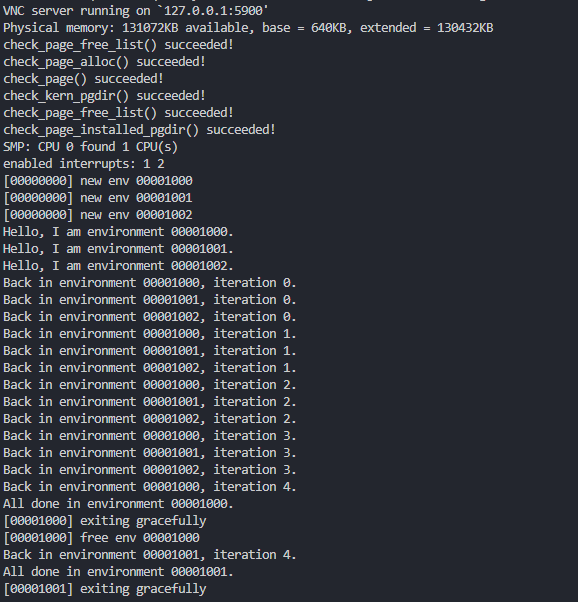
\includegraphics[width=0.5\textwidth]{ex6-1} \par
}
\newpage
若以 \textsl{make qemu CPUS=2} 命令启用双核系统,得到的运行结果如下:\par 
\quad \par  
{
\centering
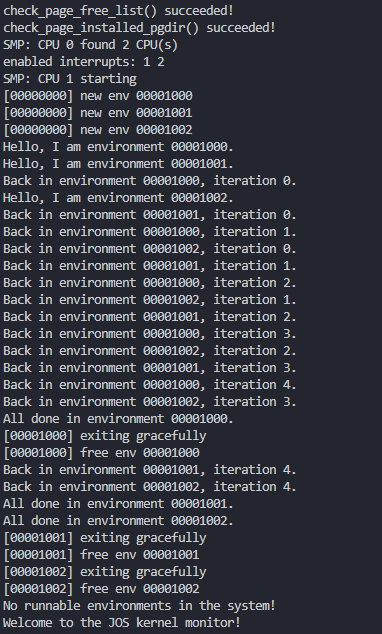
\includegraphics[width=0.5\textwidth]{ex6-2} \par
}
\quad \par 
\question{3}{
    {
        \par 
        3. In your implementation of env\_run() you should have called lcr3(). 
        Before and after the call to lcr3(), your code makes references 
        (at least it should) to the variable e, 
        the argument to env\_run. Upon loading the \%cr3 register, 
        the addressing context used by the MMU is instantly changed. 
        But a virtual address (namely e) has meaning relative to a given address 
        context--the address context specifies the physical address to which 
        the virtual address maps. 
        Why can the pointer e be dereferenced both before and after the addressing switch?
    }
    {
        \par 
        4. Whenever the kernel switches from one environment to another, 
        it must ensure the old environment's registers 
        are saved so they can be restored properly later. 
        Why? Where does this happen?
    }
}

第一个问题的答案很简单:所有的进程都映射了完整的VAS的内核部分,而envs的映射也位于内核
部分中,故所有进程对于envs数组任一进程的地址翻译都是相同的。\par 
第二个问题:进程的现场保存发生在 \_alltrap 过程中,现场恢复发生在 env\_pop\_tf() 时。


\end{document}